\documentclass[aspectratio=43,mathserif,xcolor={usenames,dvipsnames,svgnames,table},10pt]{beamer}

\usetheme[titleformat frame=smallcaps]{metropolis}
\usepackage{appendixnumberbeamer}
\usepackage{booktabs}
\usepackage[utf8]{inputenc}

\usepackage{graphicx}
\usepackage{multimedia}

\usepackage{tikz}
\usetikzlibrary{arrows}
% \usetikzlibrary{arrows.meta}
\usetikzlibrary{positioning,calc}
\usetikzlibrary{decorations.pathreplacing}
\usetikzlibrary{decorations.markings}
\usetikzlibrary{fit}
\usetikzlibrary{shapes.callouts}
\usetikzlibrary{shapes.geometric}
\usetikzlibrary{matrix}
\usetikzlibrary{spy}
\setbeamertemplate{caption}{\raggedright\insertcaption\par}
\renewcommand{\footnotesize}{\tiny}
\newcommand{\norm}[1]{\left\lVert #1 \right\rVert}
\def\doubleunderline#1{\underline{\underline{#1}}}
\usepackage{animate}
\usepackage{svg}
\beamertemplatenavigationsymbolsempty

\tikzset{
  big arrow/.style={
    decoration={markings,mark=at position 1 with {\arrow[scale=1.4]{latex}}},
    postaction={decorate},
    shorten >=2.5pt}}
\tikzset{
  big 2arrow/.style={
    decoration={markings,mark=at position 0 with {\arrow[scale=-1.4]{latex}},mark=at position 1 with {\arrow[scale=1.4]{latex}}},
    postaction={decorate},
    shorten >=2.5pt}}

\tikzset{onslide/.code args={<#1>#2}{%
  \only<#1>{\pgfkeysalso{#2}} % \pgfkeysalso doesn't change the path
}}

\pgfdeclarelayer{background}
\pgfdeclarelayer{foreground}
\pgfsetlayers{background,main,foreground}

% 
\usepackage[style=numeric,natbib]{biblatex}
\addbibresource{references.bib}

\title[NMT]{Neural Machine Translation}
\author[Arul Selvam Periyasamy]{Arul Selvam Periyasamy}
\institute[University of Bonn]{Rheinische Friedrich-Wilhelms-Universit\"at Bonn\\
Seminar: Natural Language Processing}

\date{\today}
% \logo{\includegraphics[width=2.5cm]{images/ais_uni_logo.eps}}

\begin{document}

\maketitle


\begin{frame}{Agenda}
 \begin{itemize}
  \item<+-> Introduction to Machine Translation
  \item<+-> Statistical Phrase-Based Translation
  \item<+-> Introduction to Deep Learning
  \item<+-> Neural Machine Translation

 \end{itemize}
\end{frame}

\begin{frame}{Motivation}
\begin{itemize}
 \item<+-> Translation: The process of translating words or text from one language into another (OED).
 \item<+-> Machine Translation: Translation carried out by a computer (OED).
 \item<+-> Why do we need it?
 \item<+-> Do I need to convince that we need machine translation?
\end{itemize}
\end{frame}


\begin{frame}{Machine Translation}

In a probabilistic perspective, machine translation can be formulated the problem of finding a target sentence $y$ that maximizes the conditional probability of $y$ from a given source sentence $x$.

$$ arg\,max _{y}  \,\, p(x|y)$$
\end{frame}


\begin{section}{Introduction to Deep Learning}
\end{section}

\begin{frame}{Machine Learning (Supervised)}
 \begin{figure}[h]
    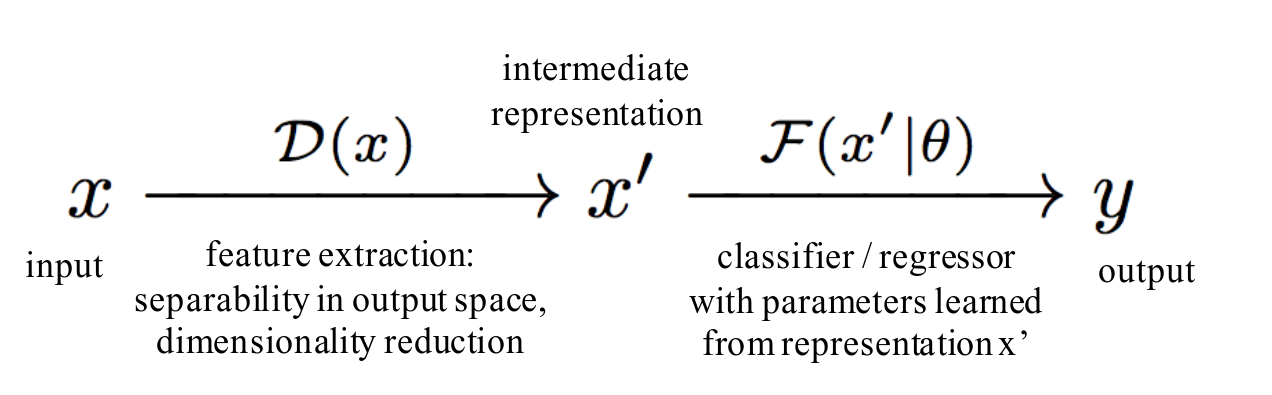
\includegraphics[width=0.9\linewidth]{images/ml.png}  
    \caption{Traditional Supervised learning}
  \end{figure}
\end{frame}


\begin{frame}{Deep Learning (Supervised)}
 \begin{figure}[h]
    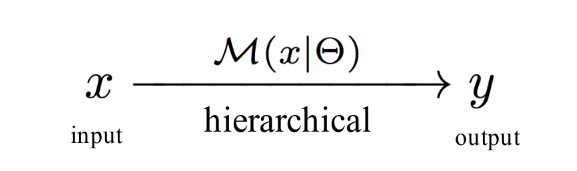
\includegraphics[width=0.9\linewidth]{images/dl.png}  
    \caption{Deep learning}
  \end{figure}
 \begin{itemize}
  \item<+-> Hierarchical representations of features.
  \item<+-> Joint learning of representation.
  \item<+-> Increased levels of abstraction.
 \end{itemize}
\end{frame}

\begin{frame}{Perceptron}
 \begin{figure}[h]
    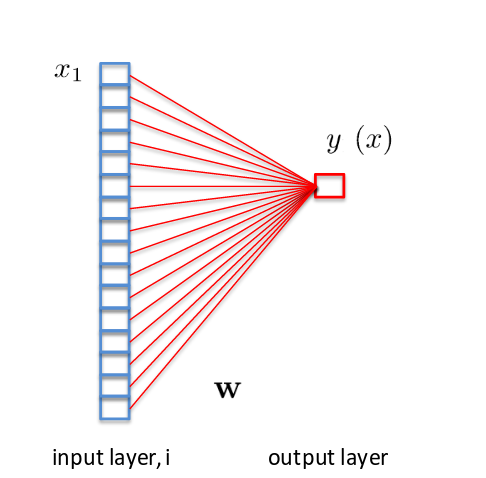
\includegraphics[width=0.5\linewidth]{images/perceptron.png}  
    \caption{A perceptron (close to a biological neuron)}
  \end{figure}
  $$ y(x) = f( W^T x )$$
\end{frame}

\begin{frame}{Logistic Regression}
 \begin{figure}[h]
    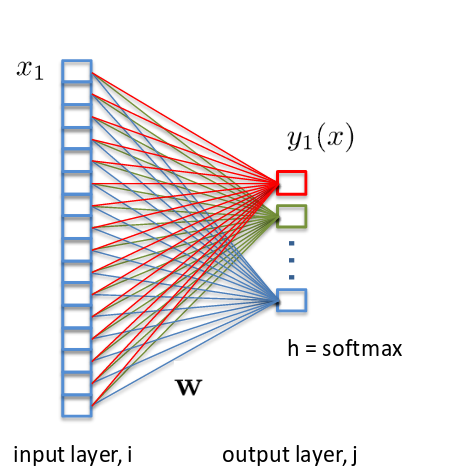
\includegraphics[width=0.5\linewidth]{images/lr.png}  
    \caption{A perceptron (A collection of perceptrons)}
  \end{figure}
\end{frame}

\begin{frame}{Logistic Regression}
Binary classification:
$$P(y = 1 | x) = h_w(x) = \frac{1}{1 + exp(-W^T x)}$$
$$P(y = 0 | x) = 1 - h_w(x) = 1 - P(y = 1 | x)$$
\end{frame}

\begin{frame}{Logistic Regression}
 Cost function: 
 $$ J(w) = - \sum_{i} ( y^i log(h_w(x^i)) + (1 - y^i) log(1 - h_w(x^i))  ) $$
 Learning Weights : Gradient Descent
 $$\nabla_w J(w) = \frac{\partial J(w)}{\partial w_j} = \sum_i x^i_j (h_w(x^i) - y^i) $$
\end{frame}

\begin{frame}{Gradient Descent}
\begin{figure}[h]
    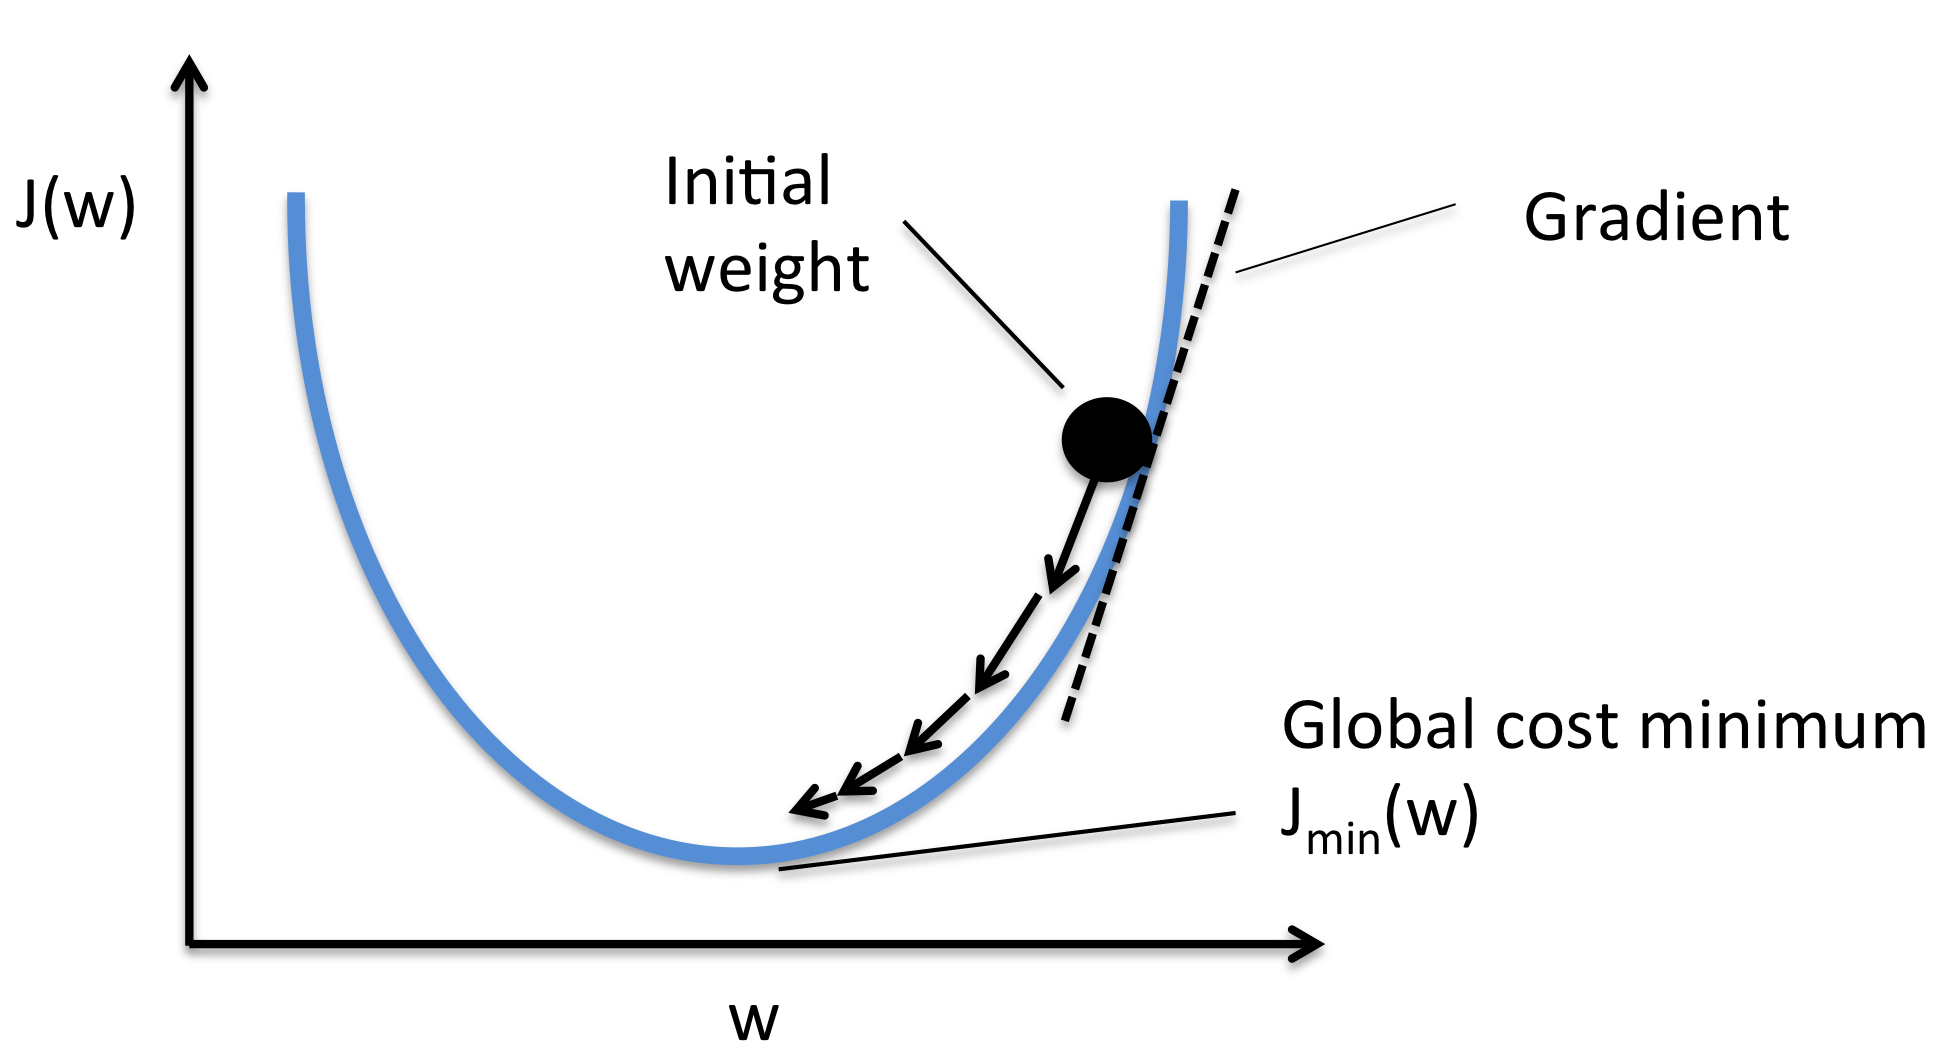
\includegraphics[width=0.7\linewidth]{images/gd.png}  
    \caption{Update weights in the direction of negative gradient.}
  \end{figure}
\end{frame}

\begin{frame}{Multi Layer Perceptron}
\begin{figure}[h]
    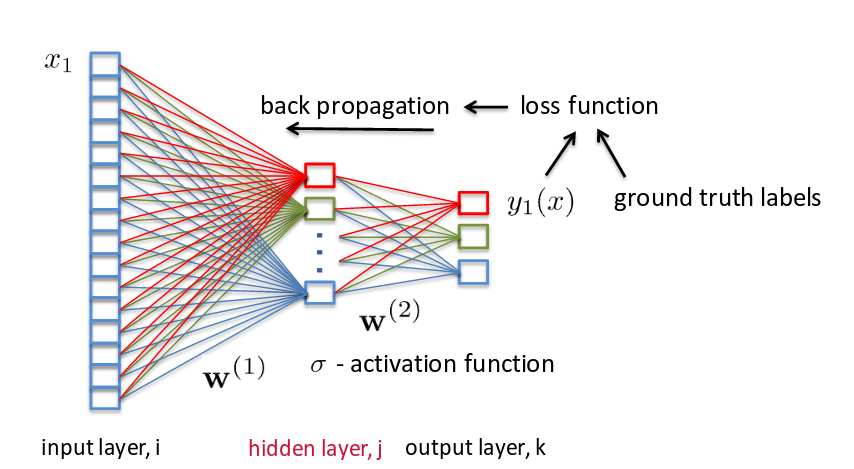
\includegraphics[width=0.7\linewidth]{images/mlp.png}  
    \caption{Multiple layers of perceptron}
  \end{figure}
  Learning weights: Same as before but apply chain rule.
  $$ \frac{\partial x}{\partial y}  = \frac{\partial x}{\partial z} * \frac{\partial z}{\partial y} $$
\end{frame}

\begin{frame}{Deep Neural Networks}
 \begin{figure}[h]
    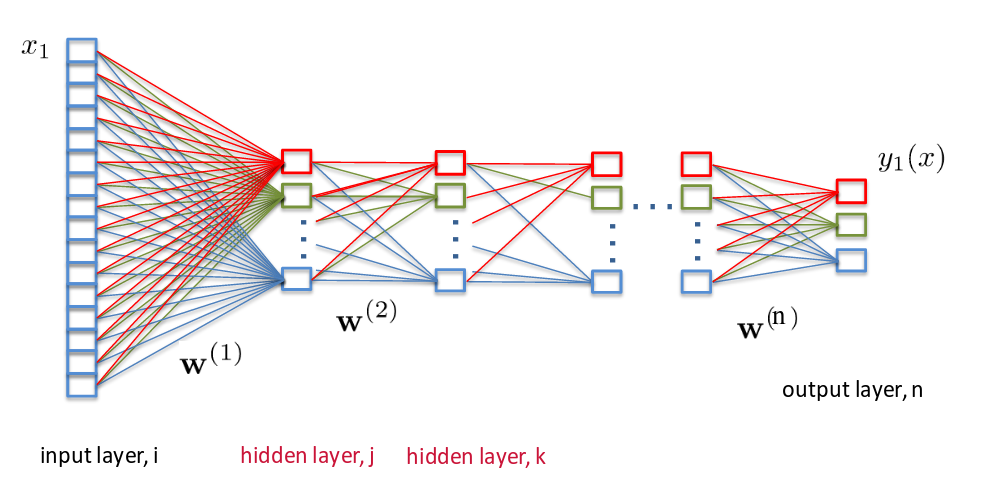
\includegraphics[width=0.7\linewidth]{images/dnn.png}  
    \caption{Deep Neural Networks}
  \end{figure}
  \begin{itemize}
   \item<+-> Simply adding layers won't work.
   \item<+-> Too many parameters to train.
   \item<+-> Need smart architectures to capture additional priors.
   \item<+-> Two most commonly used architectures are CNNs and RNNs.
  \end{itemize}
\end{frame}

\begin{frame}{Convolutional Neural Networks}
\begin{figure}[h]
    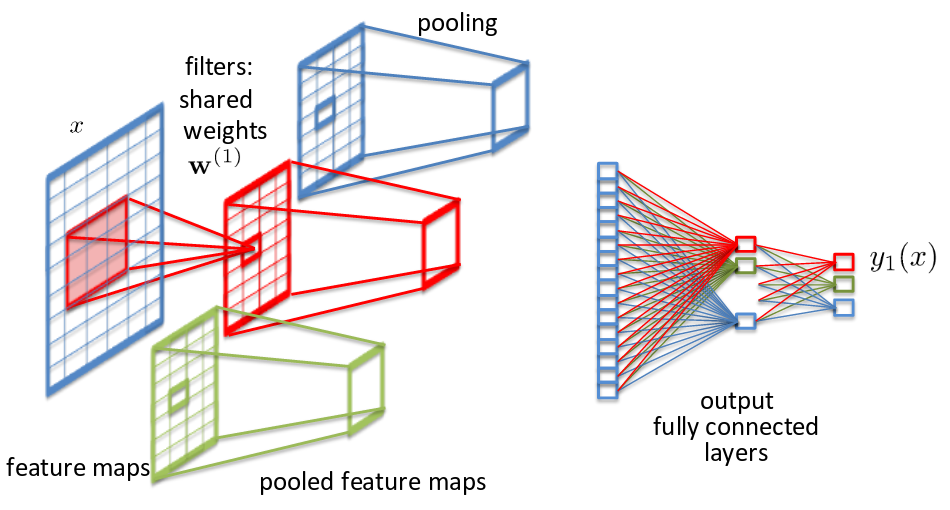
\includegraphics[width=0.7\linewidth]{images/cnn.png}  
    \caption{Convolutional Neural Networks}
  \end{figure}
\begin{itemize}
\item<+-> Each layers learns a set of convolution kernels.
\item<+-> Captures a very important prior --smoothness prior-- known to computer vision community for a very long time.
\item<+-> Much less number of parameters.
\end{itemize}
\end{frame}

\begin{frame}{Recurrent Neural Networks}
\begin{figure}[h]
    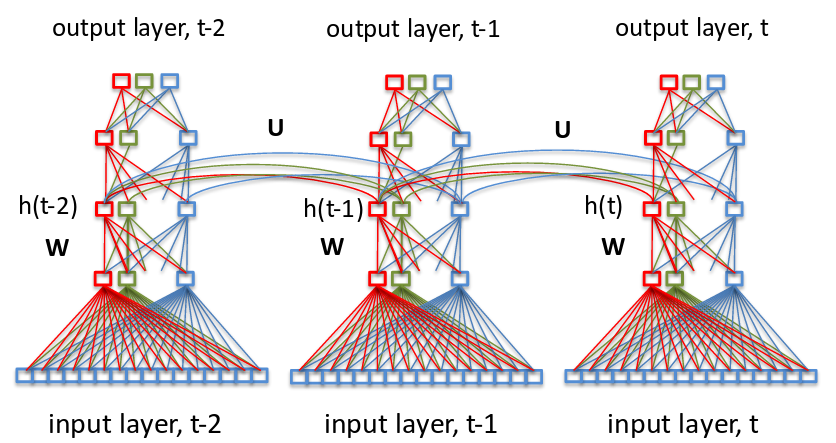
\includegraphics[width=0.7\linewidth]{images/rnn.png}  
    \caption{Recurrent Neural Networks}
  \end{figure}
  
\begin{itemize}
\item<+-> Used for predicting sequential data 
\item<+-> Captures dependences across time frames.
\item<+-> Usually harder to train (Vanishing Gradients).
\end{itemize}

\end{frame}


\begin{frame}{LSTM}
 \begin{figure}[h]
    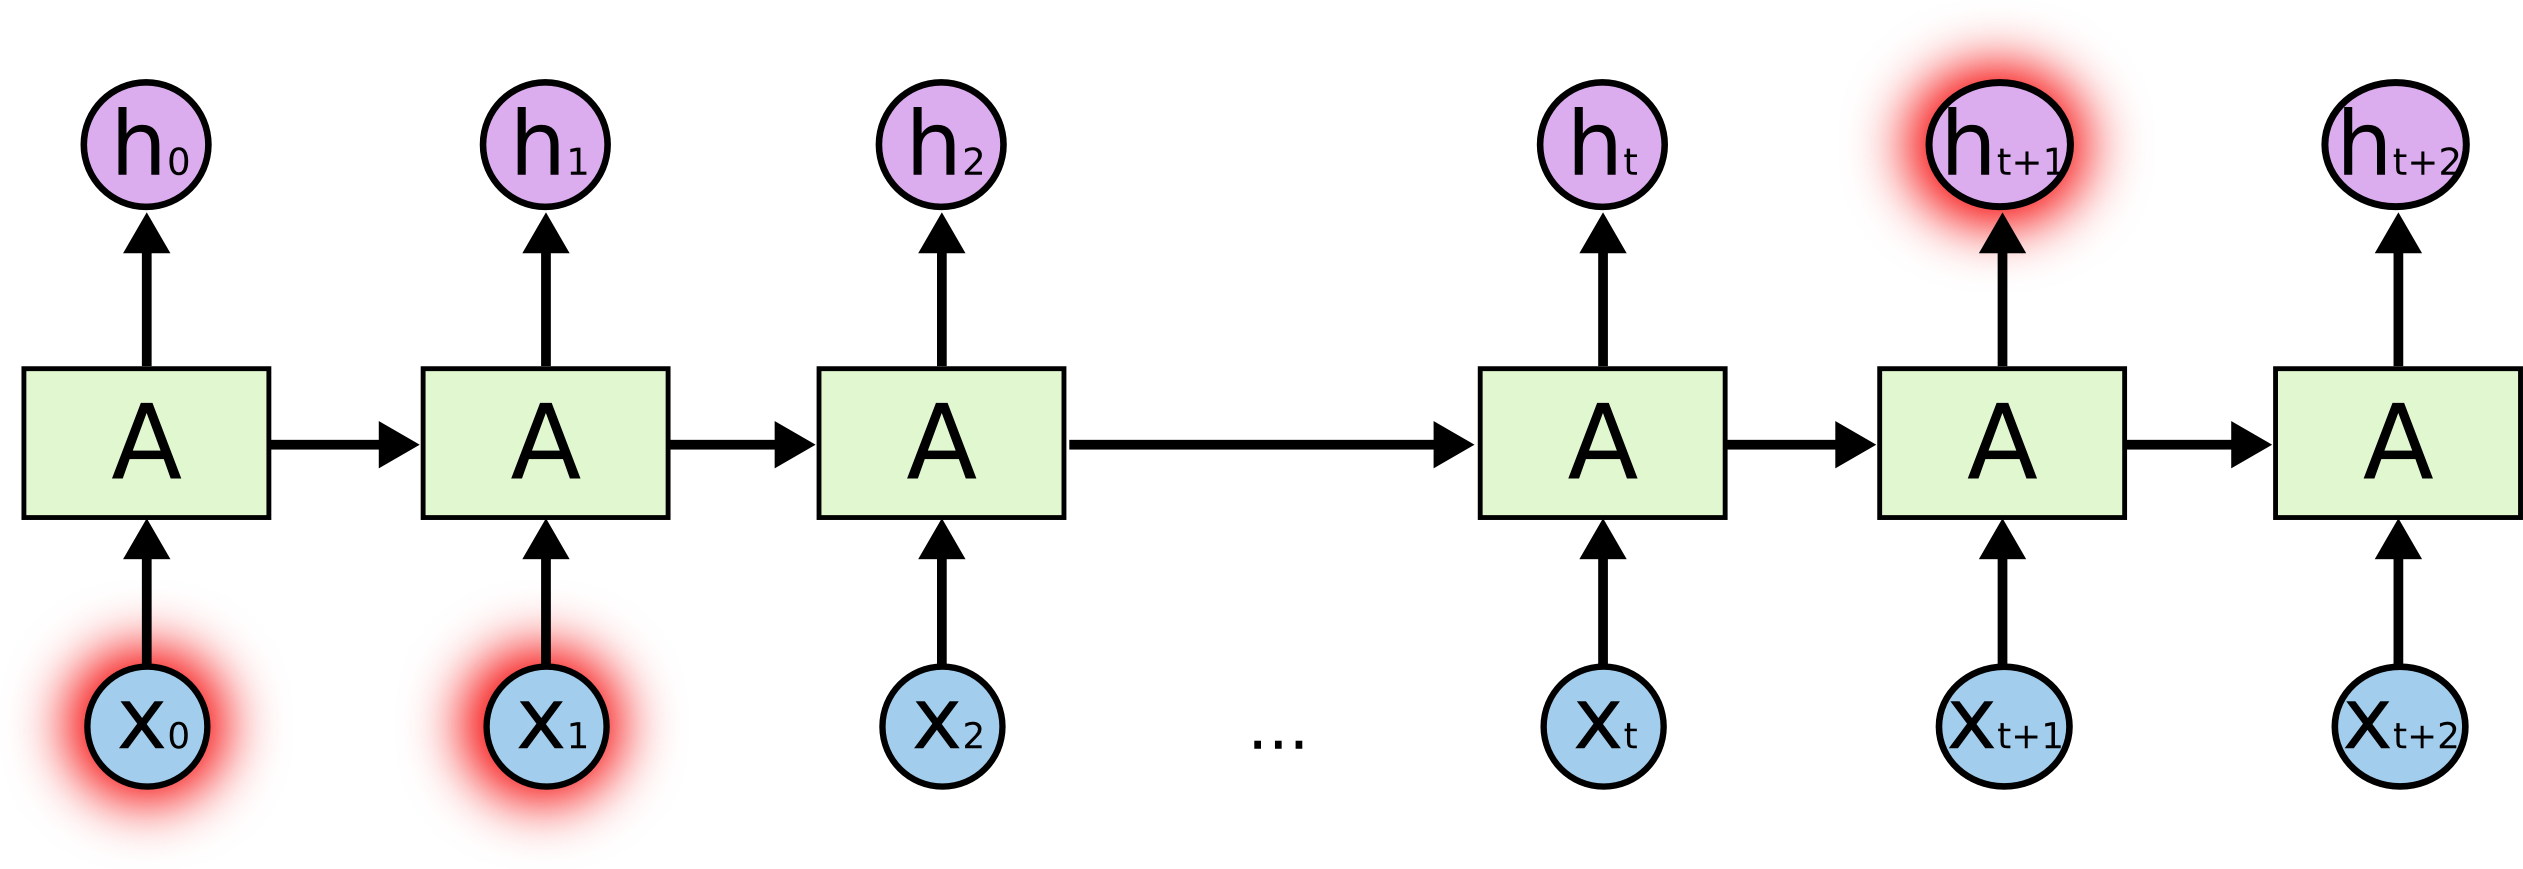
\includegraphics[width=0.4\linewidth]{images/rnn_n.png}  
    \caption{Recurrent Neural Networks}
  \end{figure}
   \begin{figure}[h]
    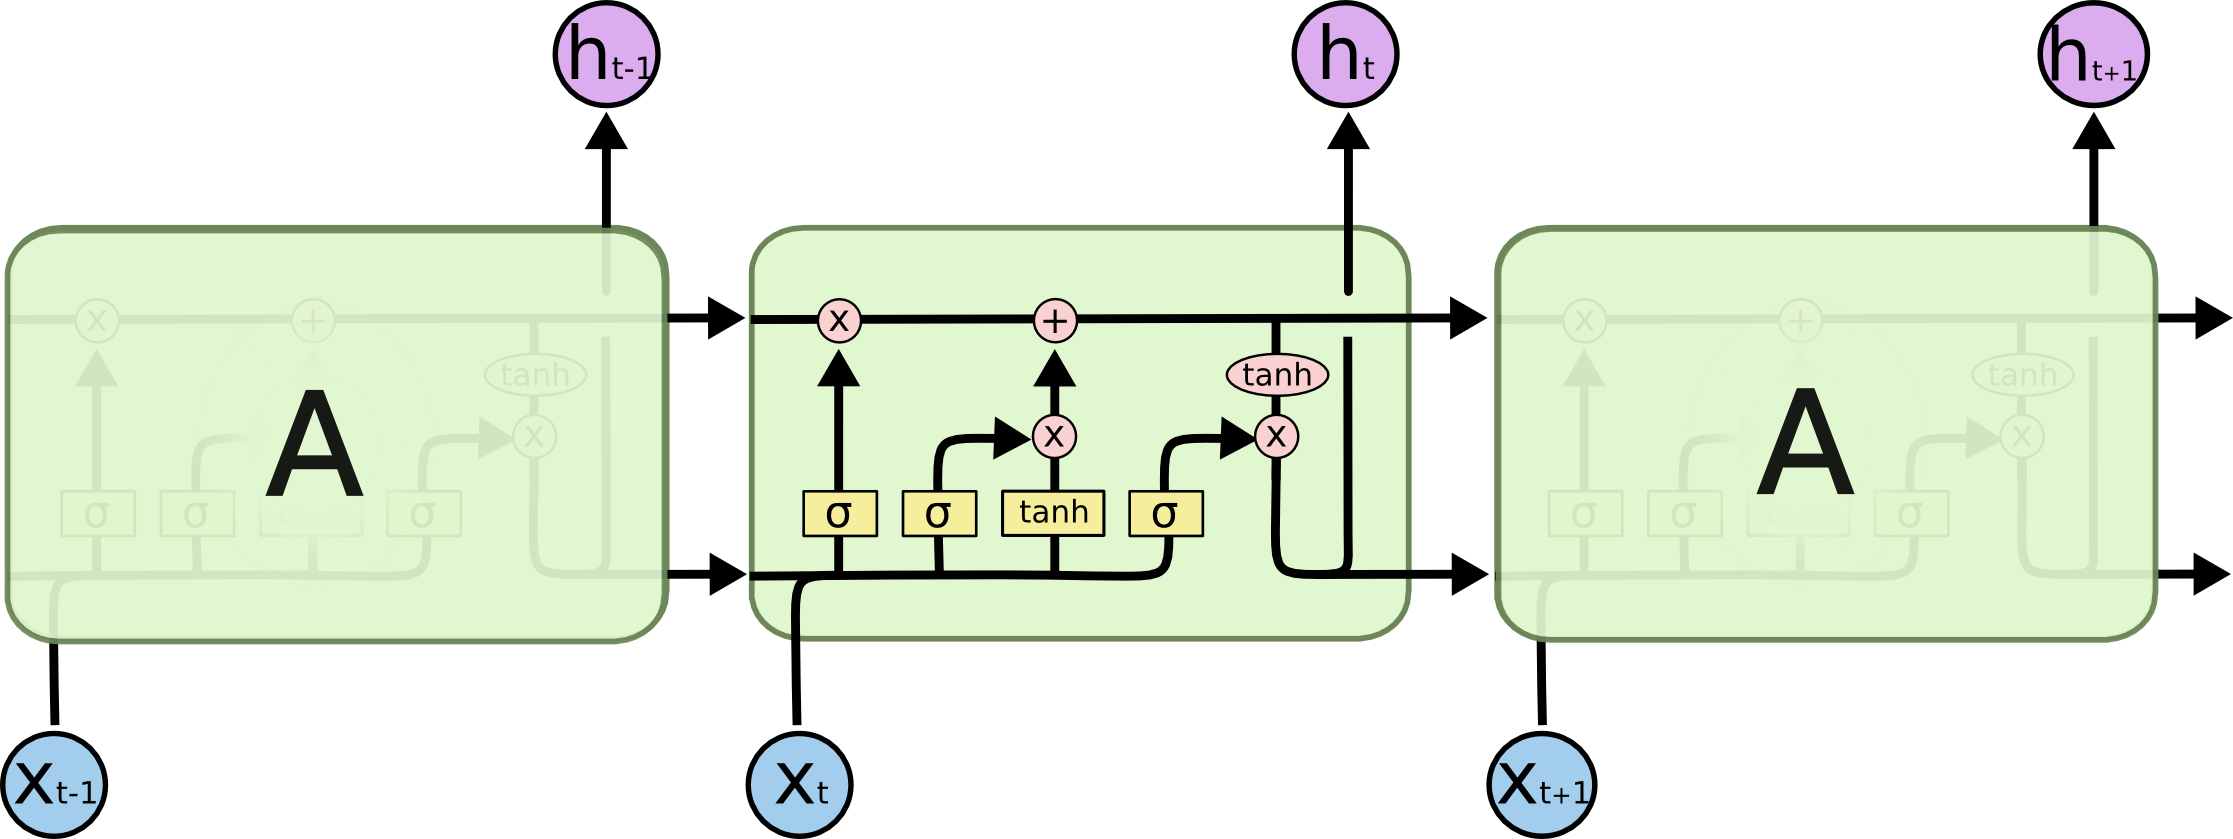
\includegraphics[width=0.6\linewidth]{images/lstm.png}  
    \caption{Long Short Term Memory}
  \end{figure}
\end{frame}


\begin{frame}{LSTM}
 \begin{figure}[h]
    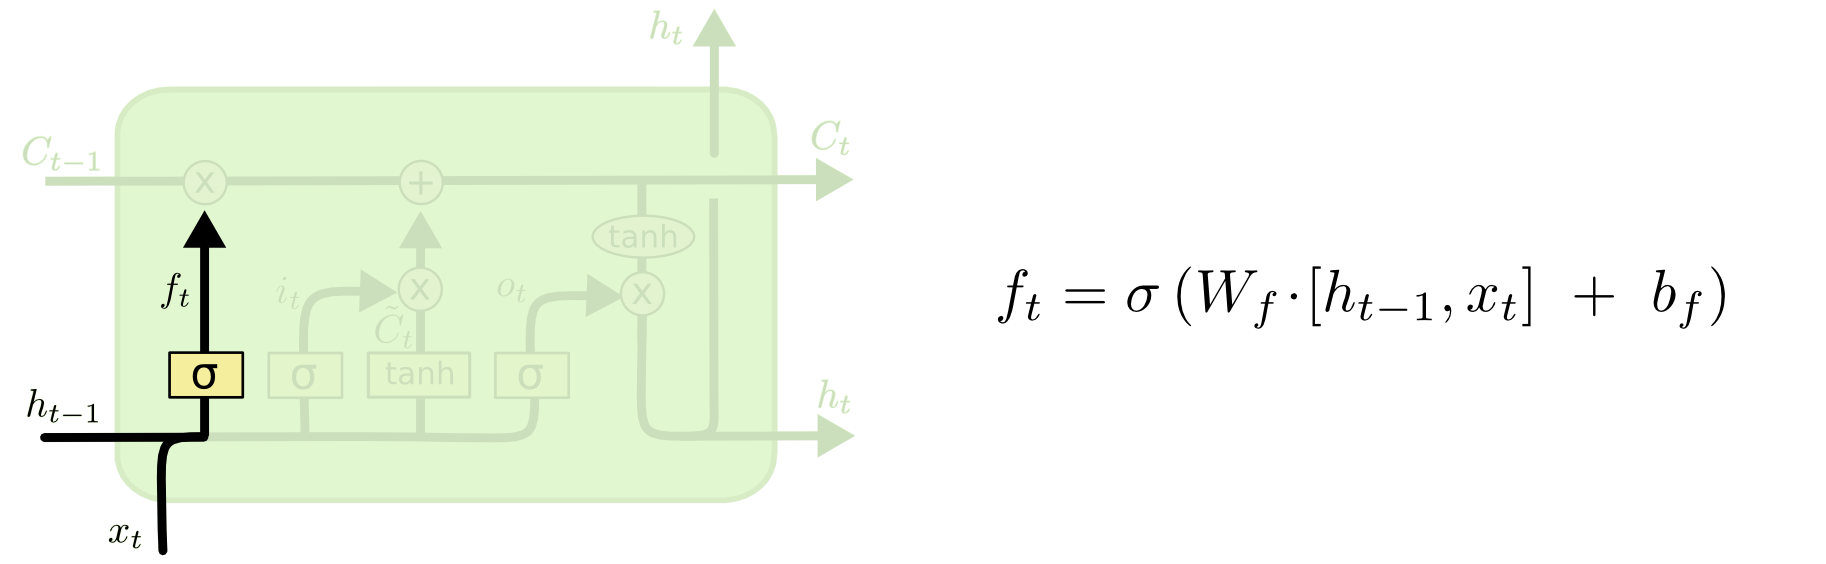
\includegraphics[width=0.6\linewidth]{images/lstm_forget.png}  
    \caption{LSTM Forget gate}
  \end{figure}
   \begin{figure}[h]
    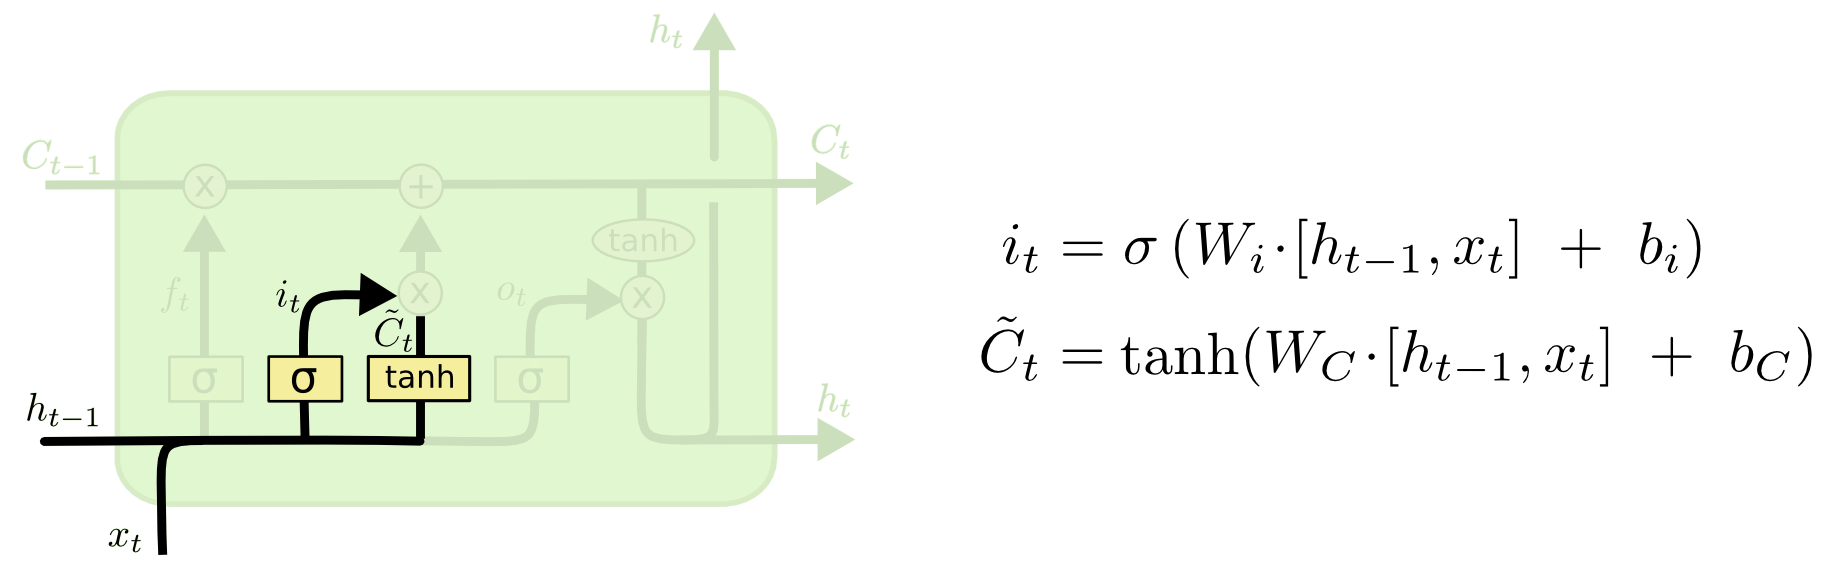
\includegraphics[width=0.6\linewidth]{images/lstm_add.png}  
    \caption{LSTM new content}
  \end{figure}
\end{frame}


\begin{frame}{LSTM}
 \begin{figure}[h]
    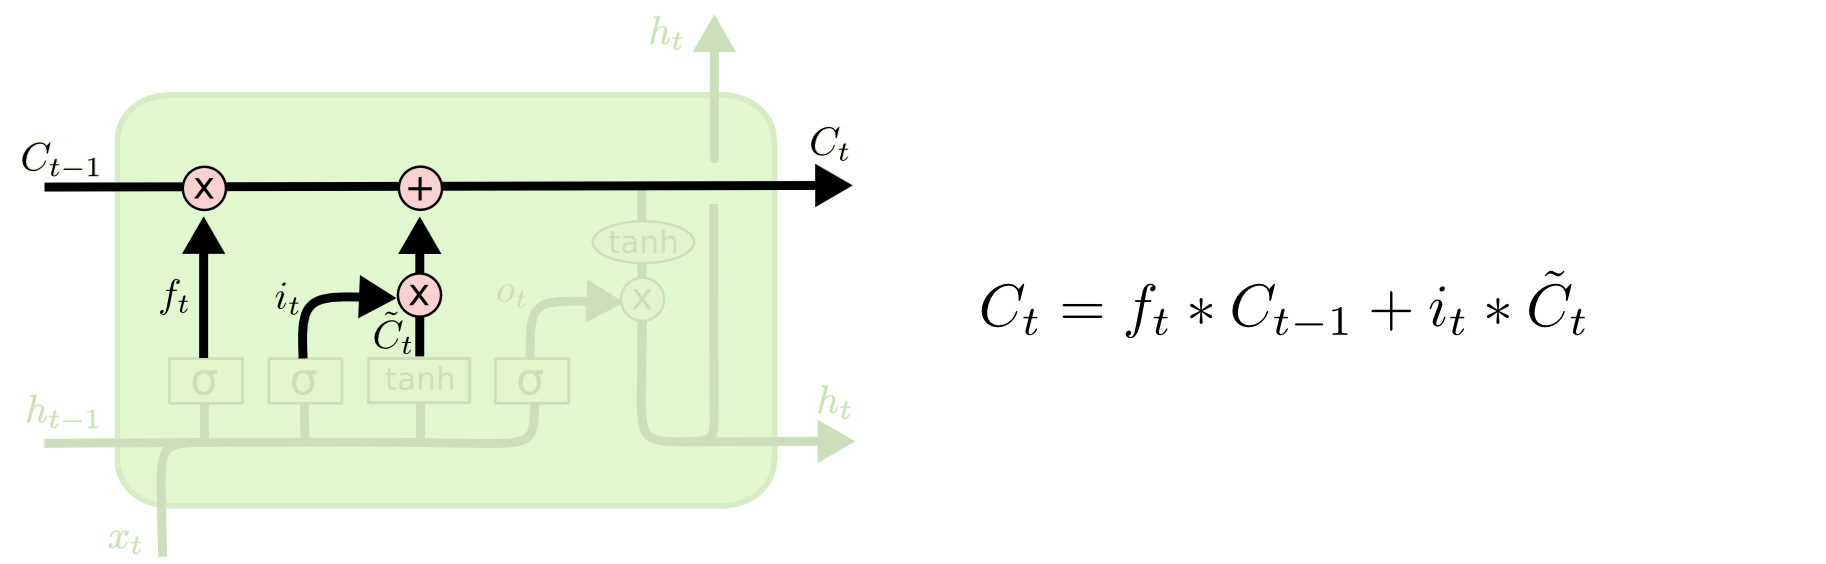
\includegraphics[width=0.6\linewidth]{images/lstm_add1.png}  
    \caption{LSTM Add gate}
  \end{figure}
   \begin{figure}[h]
    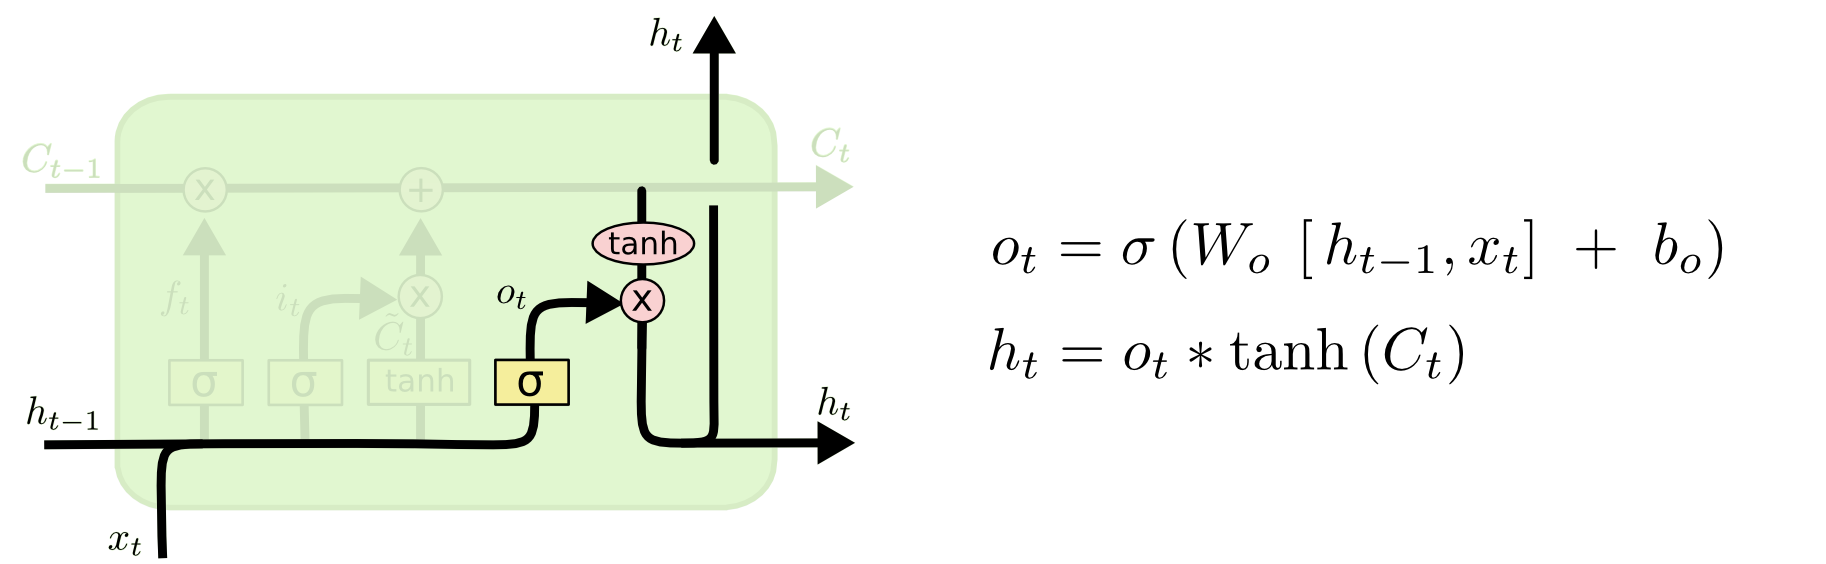
\includegraphics[width=0.6\linewidth]{images/lstm_output.png}  
    \caption{LSTM Output Gate}
  \end{figure}
\end{frame}


\begin{section}{Neural Machine Translation}
\end{section}

\begin{frame}{Neural Machine Translation}
 $$ arg\,max _{y}  \,\, p(x|y)$$
 In Neural Machine Translation, a parameterized model (a neural network) is trained to maximize the conditional probability of the sentence pairs given parallel training corpus.
\end{frame}

\begin{frame}{NMT - A historic perspective}
  \begin{figure}[h]
    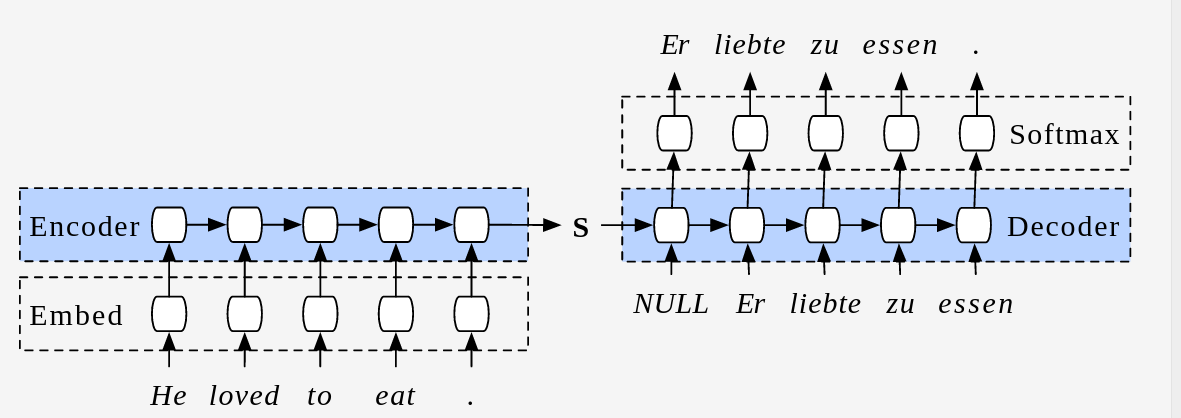
\includegraphics[width=0.9\linewidth]{images/enc_dec.png}  
    \caption{Encoder-Decoder model for Machine Translation}
  \end{figure}
\begin{itemize}
 \item<+-> Fixed size encodings.
 \item<+-> Each language typically required an Encoder and Decoder.
\end{itemize}
\end{frame}

\begin{frame}{Jointly learning to Align and translate}
\begin{figure}[h]
    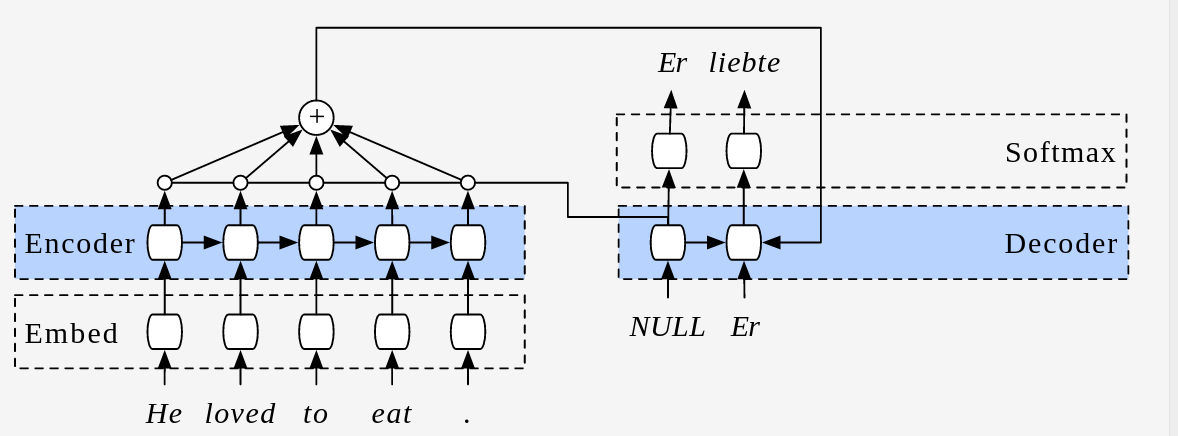
\includegraphics[width=0.9\linewidth]{images/context.png}  
    \caption{Encoder-Decoder model with context}
  \end{figure}
\end{frame}

\begin{frame}{Jointly learning to Align and translate}
For a input sentence, $X = (x_1,\cdots, x_{T_{x}} )$. The NMT \footfullcite{NEURAL MACHINE TRANSLATION BY JOINTLY LEARNING TO ALIGN AND TRANSLATE. Dzmitry Bahdanau, KyungHyun Cho, Yoshua Bengio, ICLR, 2015}
system consists of,
  \begin{itemize}
   \item<+-> Encoder and Decoder are multi-layer recurrent neural networks (RNNs).
   \item<+-> Encoder RNN, at each input step t, generates hidden state, $h_t = f(x_t, h_{t-1})$.
   \item<+-> Context vector encodes the input sequence as, $c = q(\{h_1,\cdots,h_{T_x}\})$.
  \end{itemize}
\end{frame}

\begin{frame}{Jointly learning to Align and translate}
\begin{itemize}
 \item The decoder is trained to predict the next work $y_t$ given the context vector $c$ and all previously predicted words $\{ y_1, \cdots, y_{t-1}\}$
 $$ p(y) = \prod^{T}_{t=1} p(y_t | \{ y_1, \cdots, y_{t-1}\} ,c ) $$
 \item With RNN, each conditional probability is modeled as,
 $$ p(y_t | \{ y_1, \cdots, y_{t-1}\}, c) = g(y_{t-1}, s_t, c) $$ where $s_t$ is the hidden state of the RNN.
 \end{itemize}

\end{frame}


\begin{frame}{Context Vector}
  The context vector for a input sentence $i$, is computed as a weighted sum of hidden states of the encoder (also known as \textbf{annotations})
  $$ c_i = \sum_{j=1}^{T_{x}} \alpha_{ij} h_j$$
  $$ \alpha_{ij} = \frac{ exp(e_{ij})}{ \sum_{k=1}^{T_x} exp (e_{ik})}$$

where,
$$ e_{ij} = a(s_{i-1}, h_j)  $$ is the alignment model that scores how well the inputs around the $j$ and the output at the position $i$ match.

A feedforward neural network is used as the alignment model and is \textbf{jointly trained} with all the NMT system as a whole.
\end{frame}

\begin{frame}{Visualization of the context}
 \begin{figure}[h]
    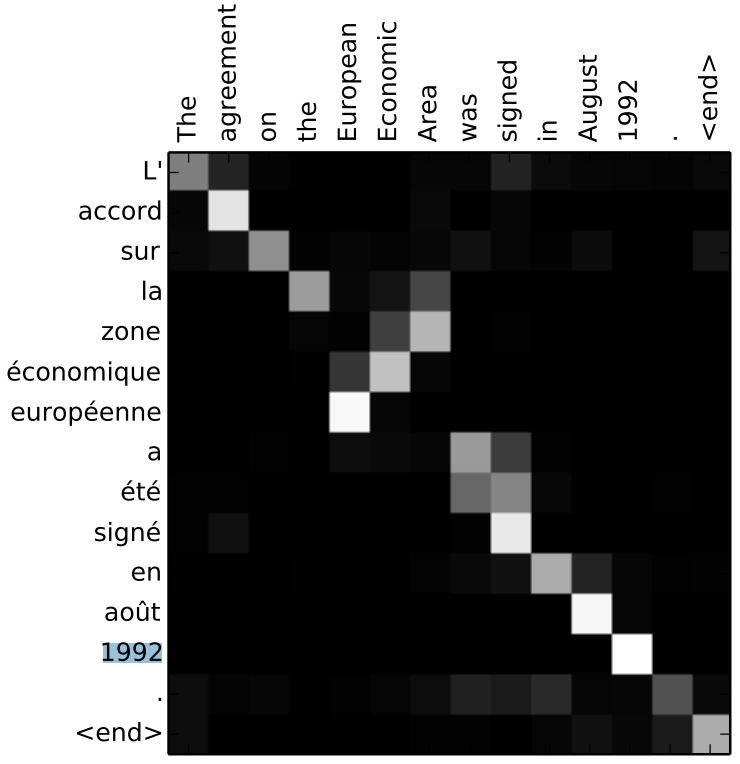
\includegraphics[height=8cm]{images/contextres.png}  
    \caption{Visualization of the context in action}
  \end{figure}
\end{frame}

\begin{frame}{Bi-directional Encoder}
 
 \begin{figure}[h]
    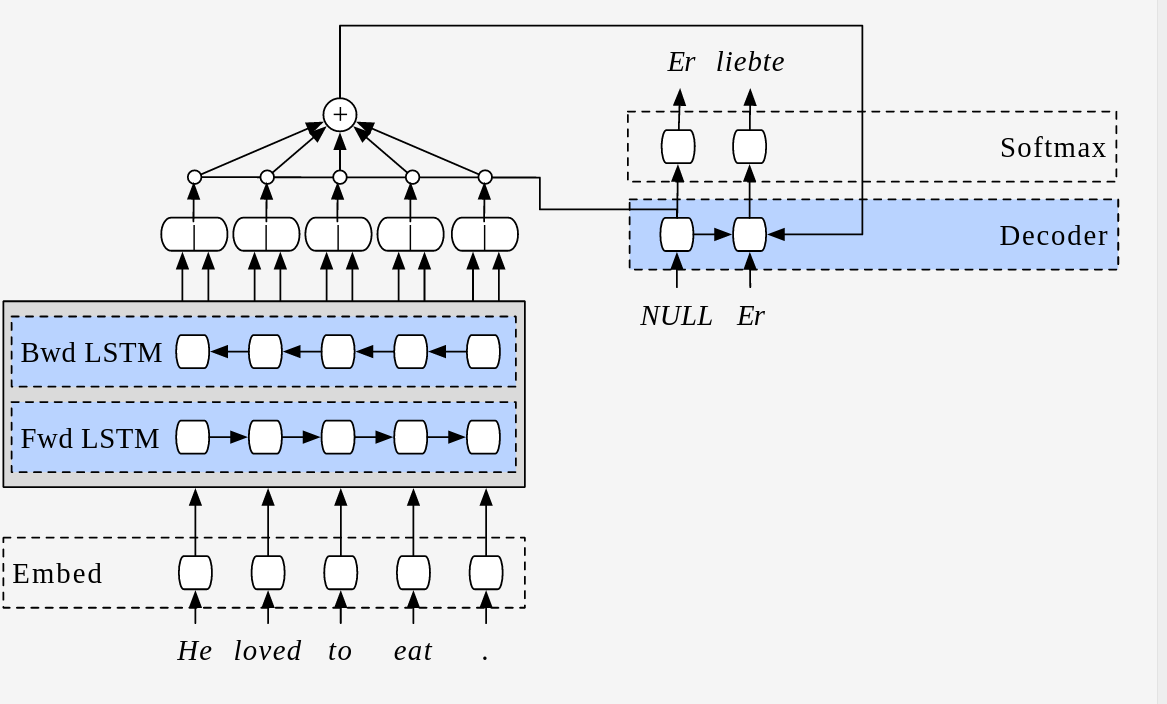
\includegraphics[width=0.9\linewidth]{images/birnn.png}  
    \caption{Bi-directional Encoder}
  \end{figure}
  \begin{itemize}
   \item<+-> Recurrent connection in both directions.
   \item<+-> Two independent states, updated independently.
  \end{itemize}
\end{frame}

\begin{frame}{Seq2Seq Learning}
 Machine Translation is can treated as a special case of a more generic sequence to sequence modeling.
 \begin{enumerate}
  \item<+-> Idea is simple: Throw more power at the network.
  \item<+-> Deep LSTM layers.
  \item<+-> No special handling for Machine translation.
  \item<+-> Trained with SGD.
 \end{enumerate}
$$ p(y_1, \cdots, y_T| x_1, \cdots, x_T) = \prod_{t=1}^{T} p(y_t| v, y_1, \cdots, y_{t-1})$$
\end{frame}


\begin{frame}{Seq2Seq Learning}
 \begin{figure}
    \centering
    \begin{tabular}{cc}
	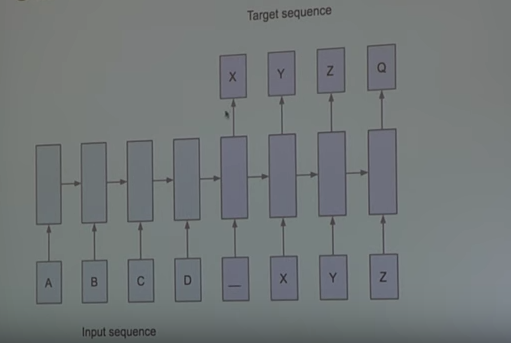
\includegraphics[width=.49\linewidth]{images/seq2seq.png} &
	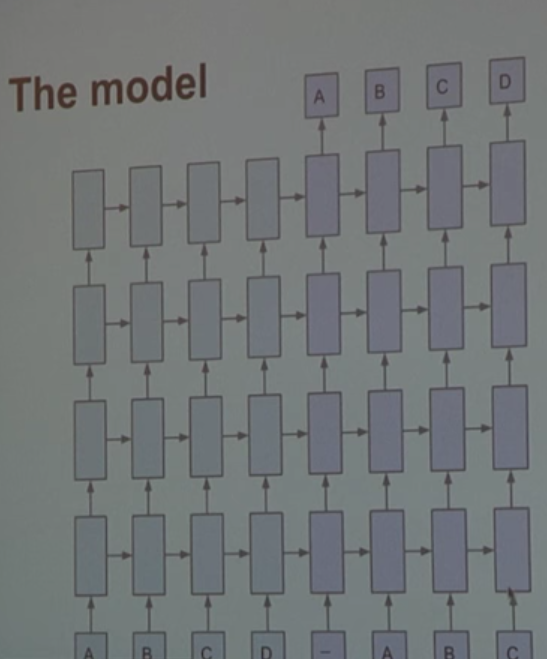
\includegraphics[width=.49\linewidth]{images/seq2seqDeep.png} \\
	\footnotesize(a) Seq2Seq model & \footnotesize(b) More powerful model \\
    \end{tabular}
    \end{figure}
\end{frame}

\begin{frame}{Seq2Seq Learning}
\begin{itemize}
 \item<+->  Trained in WMT English to French dataset with 12M sentences consisting of 348M French words and 304M English words.
 \item<+->  Used 160,000 of the most frequent words for the source language and 80,000 of the most frequent words for the target language
 \item<+->  Every out-of-vocabulary word was replaced with a special “UNK” token
\end{itemize}
\end{frame}

\begin{frame}{Seq2Seq Learning}
 Architecture details:
\begin{itemize}
 \item<+->  4 LSTM layers.
 \item<+->  1000 LSTM cells in each layer.
 \item<+->  1000 dimensional word embeddings.
\end{itemize}
\end{frame}

\begin{frame}{Google NMT}
 \begin{figure}[h]
    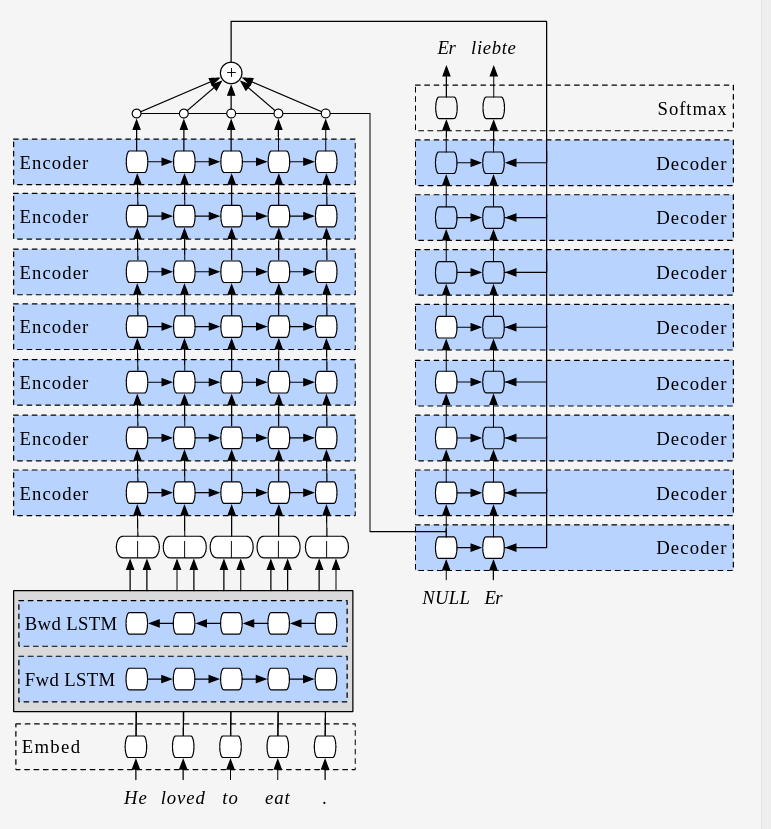
\includegraphics[height=7.5cm]{images/gnmt_1.png}  
    \caption{ Simple Encoder-Decoder but more deeper as in Seq2Seq, and Context}
  \end{figure}
\end{frame}



\begin{frame}{Residual learning}
  \begin{figure}[h]
    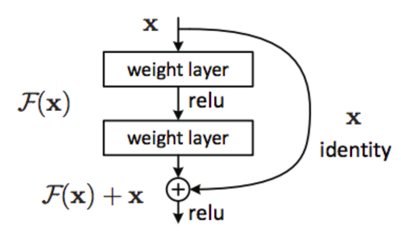
\includegraphics[width=.9\linewidth]{images/residual.png}  
    \caption{ Residual networks}
  \end{figure}
  \vspace{-1cm}
  Residual connections enables training of very deep networks. \footfullcite{Deep Residual Learning for Image Recognition. Kaiming He, Xiangyu	Zhang, Shaoqing	 Ren, & Jian Sun. CVPR, 2016}
\end{frame}

\begin{frame}{Google NMT with Residual connection}
 \begin{figure}[h]
    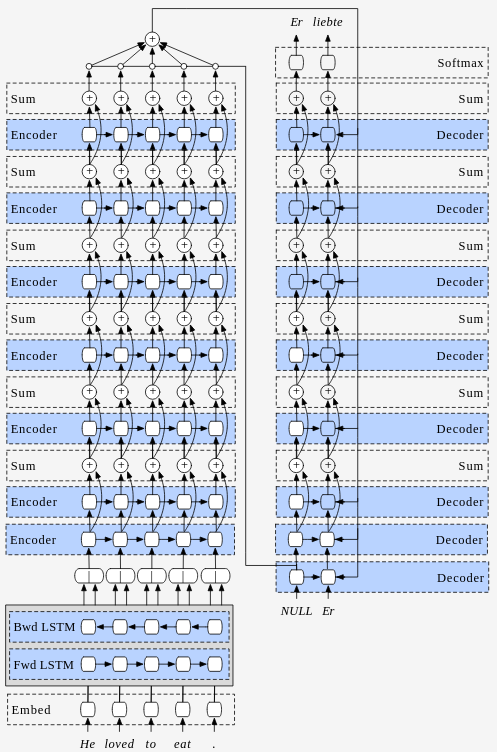
\includegraphics[height=7.5cm]{images/residual_gnmt.png}  
    \caption{ GNMT with residual connections.}
  \end{figure}
\end{frame}

\begin{frame}{Google NMT}
Google NMY properties
\begin{itemize}
 \item<+-> One Encoder and one Decoder for all the languages.
 \item<+-> The input language are encoded usign word3vec for all languages.
 \item<+-> One additional token (<__EN__>, <__FR__>, <__DE__>, <__ES__>) indicationg the target language.
 \item<+-> One gaint model that runs all Google translate queries.
\end{itemize}
\end{frame}

\begin{frame}{Conclusion}
Neural Machine Translation systems,
\begin{itemize} 
 \item Are State of the Art in Machine translation.
 \item Greatly benefited from the Neural Network research by other communities.
 \item In production by companies like Google, Microsoft, Facebook, etc.
\end{itemize}
\end{frame}



\begin{frame}{TODO}
\begin{itemize} 
 \item BLEU metric
 \item some results for all the papers
 \item PBMT
\end{itemize}
\end{frame}
\begin{frame}{References}
 http://liris.cnrs.fr/natalia.neverova/nslides/presentation_softshake_151022_novideos.pdf
\end{frame}


\end{document}